%課題研究レジュメテンプレート ver. 1.2

\documentclass[uplatex]{jsarticle}
\usepackage[top=20mm,bottom=20mm,left=20mm,right=20mm]{geometry}
\usepackage[T1]{fontenc}
\usepackage{txfonts}
\usepackage{wrapfig}
\usepackage[expert,deluxe]{otf}
\usepackage[dvipdfmx,hiresbb]{graphicx}
\usepackage[dvipdfmx]{hyperref}
\usepackage{pxjahyper}
\usepackage{secdot}

\makeatletter
  \renewcommand{\section}{%
    \if@slide\clearpage\fi
    \@startsection{section}{1}{\z@}%
    {\Cvs \@plus.5\Cdp \@minus.2\Cdp}% 前アキ
    {.5\Cvs \@plus.3\Cdp}% 後アキ
    %{\normalfont\Large\headfont\raggedright}}
    {\normalfont\raggedright}}

  \renewcommand{\subsection}{\@startsection{subsection}{2}{\z@}%
    {\Cvs \@plus.5\Cdp \@minus.2\Cdp}% 前アキ
    {.5\Cvs \@plus.3\Cdp}% 後アキ
    %{\normalfont\large\headfont}}
    {\normalfont}}

  \renewcommand{\subsubsection}{\@startsection{subsubsection}{3}{\z@}%
    {\Cvs \@plus.5\Cdp \@minus.2\Cdp}%
    {\z@}%
    %{\normalfont\normalsize\headfont}}
    {\normalfont}}
\makeatother
%ここから上を編集する必要はない.

\title{\vspace{-14mm}プレイ画像をもとにしたディープラーニングによるゲームエンジン推定}
\author{PMコース 矢吹研究室 1442045 川辺明俊}
\date{}%日付を入れる必要はない.
\pagestyle{empty}%ページ番号は振らない.
\begin{document}
\maketitle

\section{研究の背景}

現在のゲーム業界ではどのゲームエンジンを使用しているかは,基本的に公開されていない.
オープンソースのゲームエンジンであっても製作者側に使用ゲームエンジン情報を公開する義務はなく,一般人からはどのエンジンを使用しているのかは,知るすべがない.もしゲームエンジンの種類や数を詳しく知ろうとしても,そのようなデータは存在しない.

そこでディープラーニングを使用して,すでにゲームエンジンが特定されているゲームの画像情報を学習させることによって,どのゲームエンジンを使用しているか特定できるのではと考えた.

ディープラーニング(深層学習)とはニューラルネットワークの一技術であり,ニューラルネットワークはニューロンと呼ばれる脳神経を模した単位を連結されたネットワーク状のグラフである.

ディープラーニングの最も得意な分野は,画像データや波形データのような記号にできないデータの中のパターン認識だ.
入力層から画像を入力し,段階的に学習していく.
一般的によく使われているニューラルネットワークの構造は,各層をそれぞれすべて繋いでしまうパーセプトロン型だが,画像認識の場合,特殊なつなぎ型をすると比較的うまくいくことが知らている.
それを畳み込ネットワーク(コンボリューショナルニューラルネットワーク)と言う\cite{abalab}.

今回使用するディープラーニングのフレームワークはTensorFlowと呼ばれるものだ.

TensorFlowとは,Googleが開発しオープンソースとして公開した人工知能のソフトウェアライブラリである\cite{wiki}.主にできることは下記の通りである.
\begin{itemize} 
\item 顔認識
\item 画像検索
\end{itemize}

ディープラーニングのフレームワークとしてTensorFlowを使用とする理由は,Qiita(プログラマの技術情報共有サービス)での記事の数がChainerやCaffe,Theanoに比べて圧倒的に多かったからである.

\section{研究の目的}

ディープラーニングを使用して人間では特定することのできないゲームエンジン情報を特定する.

\section{プロジェクトマネジメントとの関連}

実際に使われているゲームエンジンの情報を解析することによって,新たにゲーム開発プロジェクトを開始する際に種類や数のデータが指標になりえる.

\section{研究の方法}

下記に研究の方法を記す.

\begin{enumerate}
\item CryENGINE,FOX ENGINE,Frostbite,PhyreEngine,Unity,UNREAL ENGINE の6つのゲームエンジンの画像をJPEG方式で集める.
\item 各ゲームエンジンの画像をトレーニング用に1000枚ずつ計6000枚を集める
\item 各ゲームエンジンの画像をテスト用に200枚ずつ計1200枚を集める
\item 収集したゲームエンジンの画像を読み込ませるためにテキストファイルでラベル付けをする.
\item OpenCVを使用して画像データを読み込んだ際に28×28にリサイズする.
\item TensorFlowを使用してトレーニング用に6000枚の画像を学習させて,テスト用に1200枚の画像データを読み込ませてテストデータに対する精度を表示させる.
\end{enumerate}



%\begin{wrapfigure}[行数]{r}{幅}%行数はオプションだが,調整しないとうまくいかない.
\begin{wrapfigure}[10]{r}{9cm}
\vspace*{-\intextsep}
%\includegraphics[width=図の幅,clip]{ファイル名}\label{参照用ラベル}
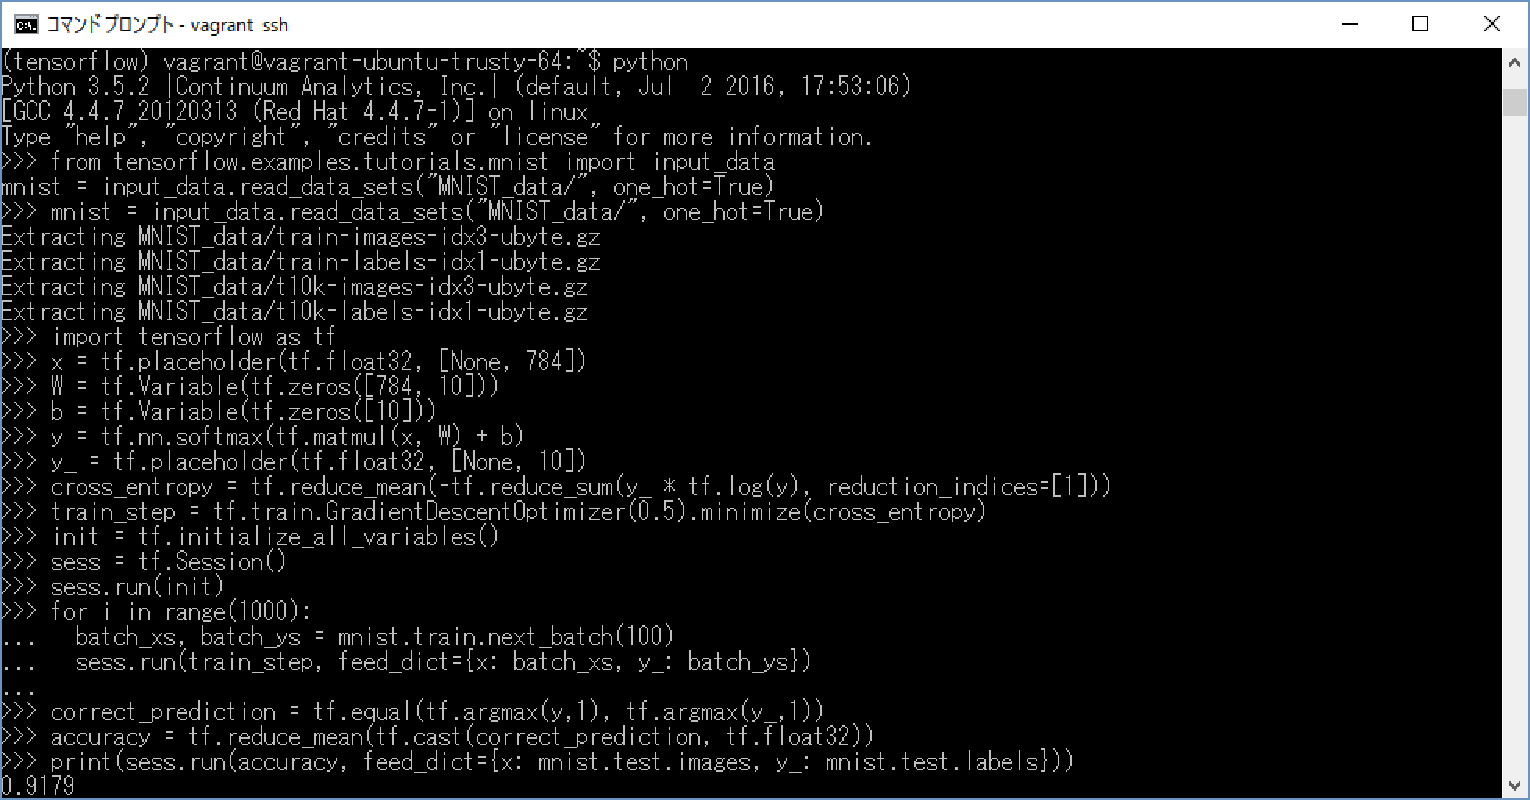
\includegraphics[width=9cm,clip]{code.pdf}
\caption{MNISTをディープラーニングで解析した時のコードと結果}\label{サンプル図}
\end{wrapfigure}


\section{現在の進捗状況}

TensorFlowのインストールを終えた後に,まずディープラーニングを試したデータはMNISTという手書きの数字の画像が入っているデータセットだ.このデータセットの中には0~9までの手書きの数字,縦28px×横28px=計784pxの訓練用データ55,000件,テスト用データ10,000件,検証データ5,000件の計70,000件が入っている.

TensorFlowを使用したディープラーニングのMNISTデータの解析の流れは,まず訓練用データ55,000件の訓練用データを学習させモデルを作成し,作成されたモデルを用いて,テスト用データ10,000件から予測された0~9のいずれかの値が算出され,その予測された値と実際の値を比較し,識別率が0.9179と出力された.

ゲームの画像を動画からコマ送りで上記で述べた枚数の画像を集めた.

TensorFlowのdecodecsvを用いて,CSVファイルでタグ付けされたJPEG形式の画像を解析し,画素の情報を3次元行列(横、縦、色面)として表現したものが得られた.

TensorFlowをインポートする際に画像の縮小の作業を請け負ってくれるOpenCVというライブラリを同時にインポートすることができなかった.その解決策としてAnaconda2とAnaconda3を同時に使用してTensorFlowとOpenCVを同時に動かすことができた.

\section{今後の計画}

今の段階で研究の方法に記してある各ゲームエンジンのディープラーニングはできてはいないから,まずはその部分を完了させる.たとえディープラーニングできるところまで行けたとしても,現在はCPUで画像の処理まで行っているので何日もの時間を奪われてしまうだろう.

そこで今後CPUで処理するのではなく,GPUでの処理が必ず必要となっていくだろうからグラフィックボードの用意が必須となっていく.

今後この実験ではゲームエンジンのトレーニング用データを学習したあと,テスト用データとの識別率が算出される.しかし現在の進捗状況に沿ってディープラーニングを行ったとしても,学習させるデータの数が少ないため,高く満足のいく識別率は算出されないだろう.

これらのことを踏まえて,以下を今後の計画とする.

\begin{enumerate}
\item 今の画像データ総数の10倍の訓練用データ60000枚,テスト用データ12000枚を集める.
\item 集めたデータをTensorFlowを使用してディープラーニングする.
\item 識別率が満足のいく数値が算出されれば,ゲームエンジンの情報が出ていないゲームの画像も解析させてデータをまとめる.
\end{enumerate}


\bibliographystyle{junsrt}
\bibliography{biblio}%「biblio.bib」というファイルが必要.

\end{document}
